\pagestyle{empty}
\documentclass[11pt]{article}
\usepackage{graphicx}
\usepackage{verbatim}
\usepackage{url}
\usepackage{graphicx, color}
\usepackage{amsmath}
%\usepackage[small,compact]{titlesec} 
%\usepackage[small,it]{caption}

\textwidth 6.5in
\headheight .1in
\topmargin -.2 in
\textheight 8.7in
\oddsidemargin 0in
\evensidemargin 1in

\begin{document} 

 \centerline{\Large \bf Blockmodels for Dynamic Network Data} 
 \medskip
\centerline{\bf Christopher DuBois}
 \bigskip

\abstract{TODO}

\section{Introduction}

Statistical methods for analyzing network data have become increasingly useful for studying  phenomenon ranging from people communicating online to protein interactions \cite{Goldenberg2009}. One class of statistical models for network data uses latent variables to help model unobserved heterogeneity.  For example, the stochastic blockmodel \cite{Nowicki2001, Kemp} assumes each node in the network belongs to some block (or cluster) and parametrizes the probability of edges between nodes of each block.  % Such approaches are especially useful for large-scale network data where higher-order dependencies can cause models such as exponential random graph models to be too complex to fit.

Network data, however, is often collected as a sequence of events occurring over time.   Recently several works have adapted models from event history analysis \cite{} to provide continuous time models of network-based event data \cite{Butts2008,Brandes2009,Perry2011,Stadtfeld2010,Stadtfeld2011,Opsahl2011,Vu2011,Vu2011a}.  These models allow one to specify how the process depends on the previous history of events.  In this way one may incorporate theories about the underlying processes and make predictions about future data conditioned on the past.

The above continuous time network models have two major drawbacks: 1) the entire network is assumed to have identical dynamics, and 2) the occurrence of any event can affect the rate at which any other event occurs.  Both aspects may be unrealistic.  Consider email communication in a small organization comprised of several teams.  Each team may have a different pattern for collaborating via email, and in many cases emails between one pair of individuals will not affect emailing behavior between a separate pair of individuals.

Borrowing from the intuition of stochastic blockmodels, we propose a hierarchical model of continuous time network data that learns latent clusters of nodes which share similar patterns of interaction.  [TODO: Explain how our experiments show that this helps.]   [TODO: perhaps use ``role'' terminology.] 
  
\section{Model}

%Each interaction then has a set of periods $d \in D_{ij}$ each with a start time $a_d$, an end time $b_d$, and a rate $\lambda_d$.
Consider a nonhomogeneous Poisson process with  intensity $\lambda(t)$ that is piecewise constant with respect to a set of knots $\tau$.  We can then write the likelihood of $M$ events as
\begin{align}
\mathcal{L}(\mathcal{A}|\theta) &= \prod_{m=1}^M \lambda(t_m) \exp\left\{ - \int_{0}^{t_M} \lambda(s)ds \right\} \\
&= \prod_{m=1}^M \lambda(t_m) \prod_{k=1}^{|\tau|} \exp\left\{ - (\tau_{k} - \tau_{k-1}) \lambda(\tau_k) \right\}
\end{align}
\noindent where the $m$th event occurs at time $t_m$, the intensity function $\lambda(t)$ is left continuous, and each $\tau_k \in [0,t_M]$.
% \begin{align}
% \mathcal{L}(A|\theta) &= \prod_{m=1}^M \lambda_{i_m}(t_m|\cdot) \prod_{i \in \mathcal{R}}  \exp\left\{ - \int_{0}^{t_M} \lambda_{i}(\tau | \cdot)d\tau \right\} \\
% &= \prod_{m=1}^M \lambda_{i_m}(t_m|\cdot) \prod_{i \in \mathcal{R}} \prod_{v \in D_{i}} \exp\left\{ - (b_v - a_v) \lambda_{i}(b_v | \cdot ) \right\}
% \end{align}

One can extend the above to marked point processes where each event contains additional information.  In the context of relational events occurring among $N$ nodes, for example, we let the \emph{risk set} $\mathcal{R}$ of possible events include all allowed dyads.  Let each dyad $(i,j) \in \mathcal{R}$ have an intensity function $\lambda_{ij}(t)$ that is piecewise constant.  We can then write the likelihood as  

\begin{align}
\mathcal{L}(\mathcal{A}|\theta) &= \prod_{m=1}^M \lambda_{i_m,j_m}(t_m|\cdot) \prod_{(i,j) \in \mathcal{R}_{i_m,j_m}}\exp\{ - (t_m - \tau_{i,j,m}) \lambda_{ij}(t_m | z_i,z_j) \}
\end{align}
\noindent where event $m$ is $(i_m,j_m)$, $\tau_{i,j,m}$ is the time  of the changepoint for $\lambda_{i,j}$ prior to the $m$th event, and $\mathcal{R}_{i,j}$ is the set of dyads who have a changepoint in their intensity when $(i_m,j_m)$ occurs. \footnote{We further assume 1) all intensity functions change at times $t=0$ and $t=t_M$, and 2) the first event is drawn uniformly from the risk set.}


\begin{figure}
 \def\svgwidth{6in}
%  \input{example1.pdf_tex}
\caption{Illustration of event data and the assumptions of the model.  Left: An sequence of two events among four nodes: (1,2) occurs at time $t_1$ and (2,3) occurs at time $t_2$.  Center: The intensity functions $\lambda_{1,2}(t)$ (solid) and $\lambda_{34}(t)$ (dotted).  Note $\lambda_{34}$ can only change when events occur involving either node 3 or node 4.  Right: Illustration of the block model, where events in cluster 1 (circles) are governed by the vector $\beta_{1,1}$, events in cluster 2 (squares) are governed by $\beta_{2,2}$, and an circle-to-square event governed by $\beta_{1,2}$.}
\label{fig:example}
%\includegraphics[width=6in]{example}
\end{figure}

For a given dyad $(i,j)$ and time $t$ we may also have a vector of statistics $\mathbf{s}(t,i,j|\mathcal{A}_t,\mathbf{z})$ that is a function of the previous event history  $\mathcal{A}_t = \{(t_m,i_m,j_m): t_m \in [0,t)\}$.   Though this will be useful, we will constrain the types of dependencies so that an interaction between one dyad does not affect the rate of an entirely separate dyad.  As shown in Figure \ref{fig:example}, we do this by assuming each intensity function $\lambda_{ij}(t)$ may only change following an event involving either $i$ or $j$.  This implies that  $\mathcal{R}_{i,j}$ is the set of dyads involving either $i$ or $j$ and that we will only use  statistics $\mathbf{s}(t,i,j)$ that do not change until an event involving either $i$ or $j$ occurs.  

We hope to learn about the dynamics between subsets of nodes while allowing for variety among disjoint subsets.   To facilitate this, we assume each node belongs to a cluster $z_i \sim \mbox{Categorical}(\alpha)$ where $\sum_k \alpha_k = 1$ and  model the intensity functions via a log linear model
\begin{align}
\log \lambda_{ij}(t | \mathcal{A}_t,\mathbf{z}) = \boldsymbol{\beta}_{z_i,z_j} \mathbf{s}(t,i,j|\mathcal{A}_t,\mathbf{z}).
\end{align}
where for each pair of clusters $(z_i,z_j)$ we have a vector of parameters $\boldsymbol{\beta}_{z_i,z_j}$ that corresponds to the covariate vector $\mathbf{s}_{ij}(t|\cdot)$.   Thus, the model of dynamics for the dyad $(i,j)$ has the same parameters as for other dyads occurring between group $z_i$ and $z_j$. 

\subsection{Model specification}

We construct $\mathbf{s}(t,i,j)$ using a similar set of statistics as used in \cite{Butts2008,Vu2011}. Let $v_{ijm} \in [0,M]$ be the index of the last event where $(i,j)$ occurred (n.b. $t_{v_{ijm}} = \tau_{ijm}$). If $(i,j)$ has never occurred, we set $v_{ijm}=0$.  
\begin{enumerate}
\item Intercept: $s_{0}(t,i,j) = 1$
\item Dyad count: $s_{1}(t,i,j) = \sum_{m:t_m<t} I(i_m=i) / m$
\item Sender out-degree: $s_{1}(t,i,j) = \sum_{m:t_m<t} I(i_m=i) / m$
\item Sender in-degree: $s_{2}(t,i,j) = \sum_{m:t_m<t} I(j_m=i) / m$
\item Receiver out-degree: $s_{3}(t,i,j) = \sum_{m:t_m<t} I(i_m=j)/m$
\item Receiver in-degree: $s_{4}(t,i,j) = \sum_{m:t_m<t} I(j_m=j)/m$
\item Reciprocity (AB-BA): $s_{5}(t,i,j) = I(i_m=i,j_m=j,i_{v_{ijm}}=j,j_{v_{ijm}}=i)$
\item Turn-taking (AB-BY): $s_{6}(t,i,j) = I(i_m=i,j_m=j,i_{v_{ijm}}=j,j_{v_{ijm}}=i)$
\item Turn-usurping (AB-XA): $s_{7}(t,i,j) = I(i_m=i,j_m=j,i_{v_{ijm}}=j,j_{v_{ijm}}=i)$
\item Turn-usurping (AB-XB): $s_{8}(t,i,j) = I(i_m=i,j_m=j,i_{v_{ijm}}=j,j_{v_{ijm}}=i)$
\item Turn-continuing (AB-AY): $s_{9}(t,i,j) =  I(i_m=i,j_m=j,i_{v_{ijm}}=j,j_{v_{ijm}}=i)$
%\item Number of shared two-paths: $s_{10}(t,i,j) =   \sum_{m:t_m<t} \sum_{r=1}^NI(i_m=i,j_m=r or i_m=r,j_m=j)$
% \item Shared contacts (since last occurrence): $s_{ij10}(t,i,j) = \sum_{r=1}^N I(i_m=i,j_m=j,i_{v_{ijm}}=i,j_{v_{ijm}}=r)$
% \item Triadic closure (since last occurrence): $s_{ij11}(t,i,j) = \sum_{r=1}^N I(i_m=i,j_m=j,i_{v_{ijm}}=r,j_{v_{ijm}}=j)$
% \item Shared contacts (since last occurrence): $s_{ij12}(t,i,j) = \sum_{r=1}^N I(i_m=i,j_m=j,i_{v_{ijm}}=r,j_{v_{ijm}}=r)$
\end{enumerate}

We include degree effects to model possible rich-get-richer phenomenon.  For example, a particular node sending often may indicate they will continue to be a sender in the future.  We normalize these counts by the number of events up until a dyad's prior changepoint.\footnote{This seems to avoid ``explosion'' when simulating from the model.  TODO: Develop some theory about these sorts of statistics.}

The next set of statistics are \emph{participation shift} effects inspired by research in conversational norms \cite{Gibson2003}.  For example, an AB-BA effect indicates an increased propensity for reciprocity.  The final set of effects allow one to model phenomenon such as triadic closure.  Though we use only the above statistics in our experiments, one may use any quantity or set of covariates about a given dyad that is computed using the previous history of events.  The only restriction is that the statistic may not change in value between each observed event.\footnote{This prevents one from using the number of events occurring in some previous time window, as in \cite{Gunawardana2011}.}

\subsection{Relation to other models}

Our formulation is reminiscent of the stochastic blockmodel \cite{Nowicki2001,Kemp} which models the probability of a dyad as $p(y_{ij}) =\mbox{logit}^{-1}( \eta_{z_i,z_j})$ where $\eta_{z_i,z_j}$ is essentially a mixing rate between group $z_i$ and group $z_j$.  Here, however, the blockmodel structure facilitates the study of intra-group and inter-group dynamics via a continuous-time network model.

The above framework generalizes several important special cases.  The first is one where events within each block share the rate at which they occur.  This can be implemented by only having an intercept statistic, $s_0(t,i,j) = 1$.  As these intensities do not change under this specification, the likelihood simplifies to 
$$\mathcal{L}(\mathcal{A}|\beta) = \prod_{m=1}^M \lambda_{i_m,j_m} \prod_{(i,j) \in \mathcal{R}} \exp\{-t_M \lambda_{i,j}\}$$
where $ \lambda_{ij} = \exp\{\boldsymbol{\beta}_{z_i,z_j}\}$.  Analogous to the stochastic block model for static networks, this model posits each dyad is a homogeneous Poisson process and all dyads within block $(z_i,z_j)$ have the intensity $\exp\{\boldsymbol{\beta}_{z_i,z_j}\}$.

\section{Inference}

We use Markov chain Monte Carlo to get samples from the posterior distribution of our parameters.  

\begin{enumerate}
\item For $i \in [1,N]$: Sample $z_i$ via Gibbs sampling: 
$z_i | A, z_{-i} \propto p(A|z,\beta) p(z_i)$.  (See Appendix.)
\item For each pair $(k,k')$: Sample $\beta_{k,k'}$ via MH or HMC.
\end{enumerate}

% TODO: Update the following discussion about sampling.

 To perform Gibbs sampling for a given cluster assignment $z_i$, we need to compute the likelihood for each possible assignment of $z_i$.   By limiting the changepoints to times when either node is involved, computing the likelihood is $O(T \cdot P \cdot 4N)$ where 4 comes from considering all dyads where either $i$ or $j$ is involved.  We precompute $\tau_{m,i,j}$ and $\mathbf{s}(t_m,i,j)$ for all $m,i,j$.  Note that 
% This operation can be done in parallel, and only the portion of the likelihood involving the newly assigned cluster  need to be recomputed.  Computing the likelihood is then $O(T \cdot P \cdot 4N)$ (though this computation is split into $K^2$ pieces) and must computed $N \cdot K$ times per Gibbs iteration.  The most straightforward implementation has space complexity $O(N^2)$ since we must keep track of $\tau_{i,j,m}$ for each $(i,j)$ at a given $m$.

% \subsection{Approximate likelihood methods}

% TODO: Discuss how one might sample the likelihood.  Cite Raftery paper.

% TODO: Look at performance of this with respect to bias and performance measure

\section{Simulation}
\begin{figure}
\center
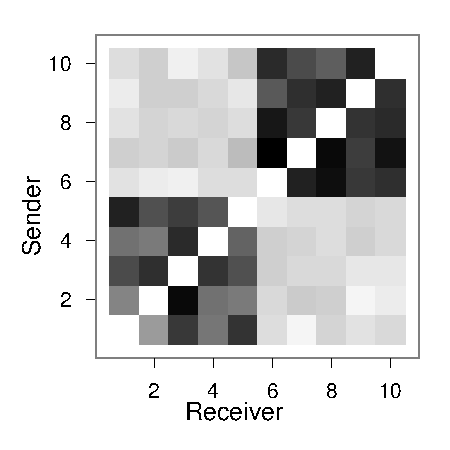
\includegraphics[width=2in]{../figs/syn/mat.pdf}
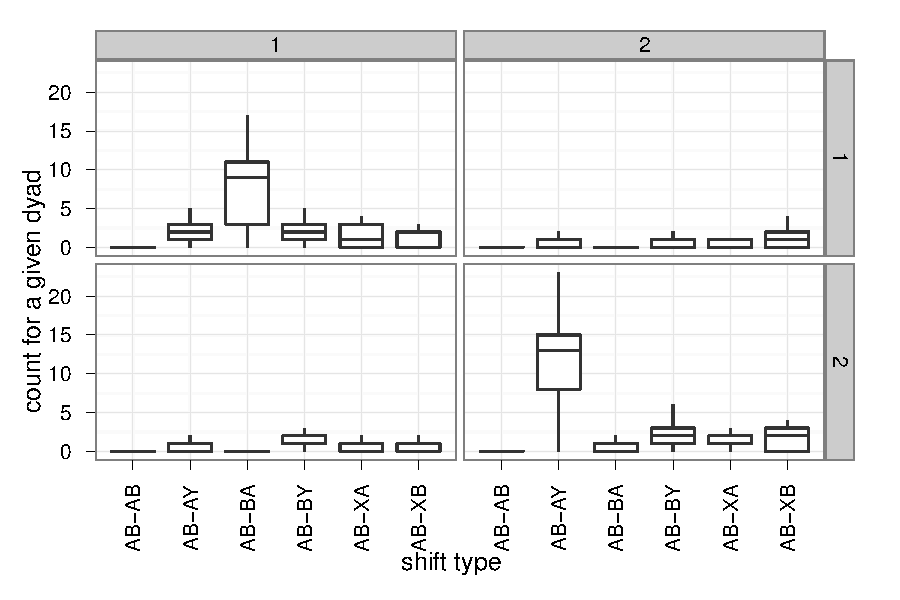
\includegraphics[width=3in]{../figs/syn/counts.pdf}
\caption{Illustration of 1000 simulated events, as described in text. Left: Counts of each dyad. Right: Boxplot of distribution of participation counts across dyads.  The top left shows an increased propensity for reciprocity within cluster 1; bottom right shows more AB-AY events within cluster 2.}
\label{fig:syncounts}
\end{figure}

We check our model fitting procedure using a small synthetic data set involving 10 nodes from 2 clusters where 1) the first cluster has an increased tendency for reciprocity, 2) members of the second cluster have an increased tendency to continue speaking, and 3) interactions between groups are more likely to be repeated.  The specification of $\textbf{s}$ is therefore $s(t,i,j) = [s_0, s_{5}(t,i,j), s_{9}(t,i,j), s_{11}(t,i,j)]$.  For the synthetic data set we use parameter vectors $\boldsymbol{\beta}_{1,1} = (2,3,0,0)$,  $\boldsymbol{\beta}_{1,2} = \boldsymbol{\beta}_{2,1} = (1,0,0,1)$, and $\boldsymbol{\beta}_{2,2} = (2,0,2,0)$.  See Appendix for details on simulating from the model.  In Figure \ref{fig:syncounts} we illustrate the simulated data and show the loglikelihood during the first iterations of MCMC [after being initialized with $\beta \sim N(\beta_{true},.5^2)$].  Note that we recover the same cluster assignments and the full model converges to the true loglikelihood.

TODO: Show parameter bias as a function of iteration; perhaps also as a function of the number of events in the dataset.

\section{Model checking and experiments}

\subsection*{Data}

Each of the following data sets are sequences of dyadic events, where each event has a time associated with it, a sender, and a recipient.

\begin{itemize}
%\item Classroom:  Perhaps within a couple of the classrooms we can infer subgroups who tend to obey different relational event dynamics.
\item Email: In small organizations there may be groups of people who tend to have a similar style of interaction, and who also share a pattern of interaction with those outside the group or in another group.
%\item Citation networks: Perhaps some groups of papers obey some types of rich-get-richer effects more than others.
\item We collected tweets from Twitter.com occurring between from May 11, 2009 to January 26, 2012 that contained the hashtag \texttt{\#rstats}.  This hashtag is used to denote messages pertaining to the R statistical computing environment and sometimes statistical discussion more generally.  We collect dyadic events by selecting tweets beginning with the \texttt{@} symbol (called a \emph{mention}), and mark the first mentioned user as the recipient.  Of 28337 total tweets in this time period, 3926 were directed events among a total of 1079 users.  We use the subset of 487 users who participated in more than one event, using a training set of 2000 events and a test set of 1330 events.
\end{itemize}

\subsection*{Prediction experiment}

\begin{figure}
\center
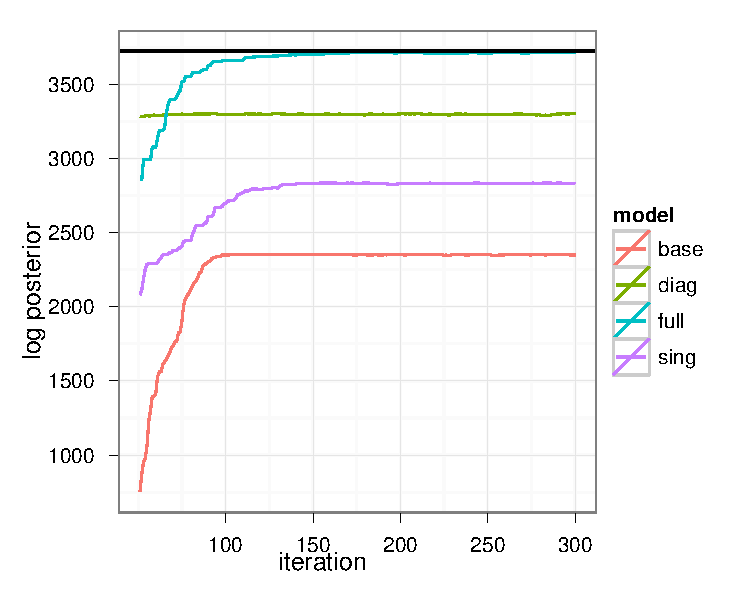
\includegraphics[width=3in]{../figs/syn/logposterior.pdf}
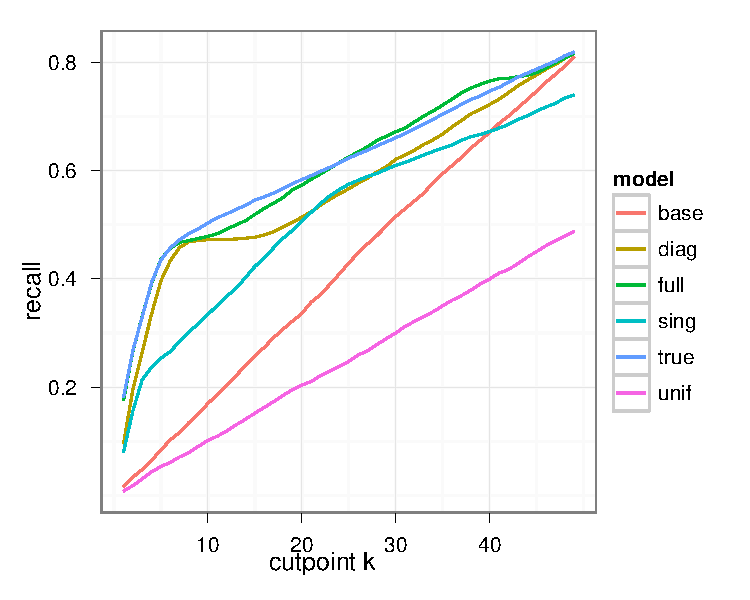
\includegraphics[width=3in]{../figs/syn/test-recall.pdf}
\caption{Results from fitting models to synthetic data. Left: Log posterior of 1000 simulated events vs. iteration during MCMC.  Right: Recall on 3000 test events.}
\label{fig:synresults}
\end{figure}
We evaluate the predictive ability of the learned models by comparing models based on the loglikelihood of held-out data and recall on held out data.  Each data set is first split into a training set and a test set, and the loglikelihood of the test set is computed using Equation \ref{eqn:llk} where $\beta$ is set to be the mean from posterior samples given the training data.  

In addition, we compute recall to evaluate whether the next observed event is among the most likely according to the model.  At each event $m$ we sort the predicted intensities of all possible events in decreasing order, find the rank of the observed event in the list of predicted intensities, and compute the mean rank across the $M$ events.  

Several baselines are included for comparison: \texttt{uniform} places uniform probability on all possible dyads, \texttt{online} ranks events at time $t$ by the number of times the dyad has occurred previously $\sum_{m:t_m < t} I(i_m=i,j_m=j)$, and \texttt{marginal} uses the product of the observed marginal frequencies $\sum_{m:t_m < t} I(i_m=i) \sum_{m:t_m < t} I(j_m=j)$.  Note for processes that are homogeneous over time, \texttt{online} should do well with large amounts of data while \texttt{marginal} should roughly model heterogeneity in activity among individuals.

We consider several variations of our model to investigate its properties. The \texttt{baserates} model only is an intercept only model (and mimics the behavior of a stochastic block model).   The \texttt{full} model uses all the statistics discussed in Section \ref{sec:modeladditional}.  For the \texttt{shared} model we force all diagonal blocks to use the same vector ($\boldsymbol{\beta}_{k_1,k_2} = \boldsymbol{\gamma}_1$ where $k_1=k_2$) and all non-diagonal blocks to use the same vector to be the same  ($\boldsymbol{\beta}_{k_1,k_2} = \boldsymbol{\gamma}_2$ where $k_1 \ne k_2$).  For each of these we may vary the number of clusters $K$. The \texttt{single} model uses all statistics but assumes a single cluster $K=1$. 

TODO: In Figure \ref{fig:} we show the recall for each dataset.

TODO: In Table \ref{tab:} we show the likelihood on the test dataset.

TODO: Need to see how well the time-portion of the model is specified.

\section{Discussion}

TODO: Discuss experimental results.  Describe qualitative behavior of each model's recall line.

TODO: Discuss any interpretation of the parameters and clusters for both datasets.

Relational event models \cite{Butts2008} require a knot at each observed event, while other approaches \cite{Gunawardana2011} aim to learn the regions where an intensity is constant and allow for a nonlinear relationship between statistics and the intensity function.  

\subsection{Extensions}
Possible future work could extend the present framework to a mixed-membership model where for each effect there is a latent cluster assignment.  This way a group of nodes might contact high in-degree nodes at a similar rate, though they vary in the degree to which they adhere to reciprocity.  As in the mixed-membership stochastic blockmodel \cite{Airoldi2008,Shafiei2010}, one could assume that each node has vector of probabilities, $\boldsymbol{\pi}_i$, for being assigned to each of the latent clusters.  In that case $z_i \sim \mbox{Categorical}(\boldsymbol{\pi}_i)$ for each node $i$ and $j$, and the ties are modeled via a stochastic blockmodel $\mbox{logit} p(y_{ij}) = \eta_{z_i,z_j}$.  One could extend our current framework by assuming that for each event $m$, any node  $i,j \in \mathcal{R}_{i_m,j_m}$ redraws their latent class.  

Possible variants:
\begin{itemize}
\item Discuss possible variations on the prior structure of $\beta$: 1. Enforce $\beta_{k,l} = \beta_{l,k}$. 2. Assume $\beta_{k,l,p} \sim \mbox{Normal}(\beta_p,\sigma_p^2)$. 3. Place other priors that provide different kinds of regularization. 
\item $\log \lambda_{ij} = (\pi_i \cdot \pi_j) \eta s(t,i,j)$
\item  HMM that guides which latent class over time?
\item  HDP instead of fixed K: Hierarchical, nonparametric model that allows parameters to be shared across blocks.
\item different clusters for senders and receivers (cite our KDD paper)?
\item More statistics, e.g. topic model similarity
\end{itemize}

\section{Conclusion}
 We propose a hierarchical approach for modeling event-based network data that is analogous to recent hierarchical extensions for latent position models \cite{Handcock2007} and exponential random graph models \cite{Schweinberger2011}.  The method combines a latent variable framework (stochastic blockmodels) with a local dependence model for event sequences (relational event models) to provide detailed models of event dynamics among subsets of nodes while simultaneously allowing for heterogeneity in dynamics of the network as a whole.


\appendix
\section{Simulation}

Simulation from the model follows the typical racing exponentials idea with a few subtleties.

\begin{enumerate}
\item $t_0 = 0$, all $s_{ij} = 1$, Initialize $v = 0$
\item For $i = 1, \ldots, N$: Draw $z_i \sim \mbox{Categorical}(\theta)$
\item For $m = 1, \ldots, M$:
  \begin{enumerate}
  \item Draw $t_m \sim \mbox{Exponential}\left(\sum_{ij} \lambda_{ij}^*\right)$
  \item Draw $(i_m,j_m) \sim \mbox{Categorical}\left(\lambda_{ij}^* / \sum_{ij}\lambda_{ij}^*\right)$
  % \item Save $s_{ij}(t_m) \leftarrow s_{ij}^*$
  % \item Save $\lambda_{ij}(t_m) \leftarrow \lambda_{ij}^*$
  \item For all $(i,j)$ where $i$ or $j$ is in $\{i_m,j_m\}$:
    \begin{enumerate}
    \item Compute $s_{ij}^*$ using event $0$ through $v_{ij}$
    \item Set $\lambda_{ij}^* \leftarrow \exp\{ \beta_{z_i,z_j} s_{ij}^*\}$ 
    \end{enumerate}
  \end{enumerate}
\end{enumerate}

\section{Gibbs sampling}

Let $\mathcal{U}_a = \{a: a \in (i_m,j_m), m \in [1,M]\}$ be the set of events where actor is involved:

$$p(A|z,\beta,a \ \mbox{involved}) = \prod_{a \in \mathcal{U}_a} \lambda_{i_a,j_a}(t_a|\cdot)
\prod_{(i,j) \in \mathcal{R}_{i_a,j_a}} \exp \{ -(t_a - \tau_{ija}) \lambda_{ij}(t_a|\cdot)\}$$

\section{EM for baseline}

In our baseline model, each block $(a,b) \in [1,K] \times [1,K]$ simply has a rate $\gamma_{a,b}$.
The likelihood is
\begin{align*}
\mathcal{L}(A|\lambda) &= \prod_{m=1}^M \lambda_{i_m,j_m} \prod_{(i,j) \in \mathcal{R}} \exp\{-t_M\lambda_{ij}\} \\
& =\prod_{a=1}^K \prod_{b=1}^K \prod_{m=1}^M \gamma_{ab}^{I(z_{i_m}=a,z_{j_m}=b)} \prod_{(i,j): z_i=a,z_j=b} \exp\{-t_M\gamma_{ab}\} \\
& =\prod_{a=1}^K\prod_{b=1}^K \gamma_{ab}^{n_{ab}} \exp\{-t_Mn_an_b\gamma_{ab}\}
\end{align*}
where $n_{ab} = \sum_m I(z_{i_m}=a,z_{j_m}=b)$, $n_a = \sum_{i=1}^N I(z_i=a)$.

The loglikelihood is $$\ell(A|\lambda) = \sum_{a=1}^K \sum_{b=1}^K n_{ab} \log \gamma_{ab} - t_M n_a n_b \gamma_{ab}$$
and so $\hat{\gamma}_{ab} = \frac{n_{ab}}{t_Mn_an_b}$.


I do not believe it is possible to perform EM for a model where we have the more general linear predictor for the intensity function.  Since the assignment of one node depends on the assignments of the other nodes, we suffer combinatorial explosion.
\bibliographystyle{plain}
\bibliography{refs}

\end{document}
